\makeatletter\let\ifGm@compatii\relax\makeatother
\documentclass[red]{beamer}

%\usepackage{beamerthemesplit}
\usepackage{listings}
\usepackage{comment}
\usepackage{url}
\usepackage{bm}
\usepackage{tikz}
\usepackage{enumitem}
\usetikzlibrary{arrows.meta}
\usetikzlibrary{shapes.symbols}

\usepackage{hyperref} % has to be last
\hypersetup{
    colorlinks=true,
    linkcolor=blue,
    filecolor=magenta,      
    urlcolor=cyan,
    pdfpagemode=FullScreen,
    }

\tikzset{
    saiarrow/.style={{-Latex}, thick}
}

\newcommand{\isred}[1]{{\color{red} {\bf #1}}} 
\newcommand{\isblue}[1]{{\color{blue}{\bf #1}}} 
\newcommand{\isgreen}[1]{{\color{green} {#1}}} 
\newcommand{\isdarkgreen}[1]{{\color{darkgreen} {#1}}} 
\newcommand{\isorange}[1]{{\color{orange} {#1}}} 

\begin{document}


\setbeamercolor{alerted_text}{fg=cyan}
\xdefinecolor{purplish}{cmyk}{0.75,0.75, 0, 0}
\xdefinecolor{purple}{cmyk}{0.75,0.75, 0, 0}
\colorlet{newred}{red!60!black}

\title{Session 4: PAKE-0, Assumptions, and Channels}
\author{Slides prepared by UMBC Protocol Analysis Lab}
\date{Last edited \today}
\begin{frame}
\maketitle
\end{frame}

\begin{frame}\frametitle{Passwords}
\centering
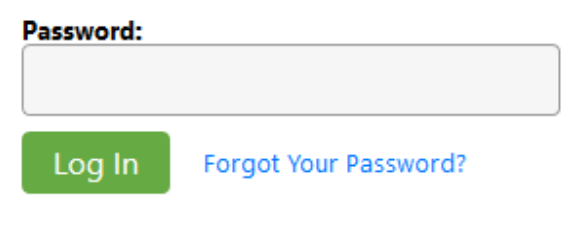
\includegraphics[width=0.5\linewidth]{slide-images/password}
\begin{itemize}
\item Can help prove your identity to somebody.
\item We've used these forever.
\item Should be kept secret and hard to guess.
\item Often memorized\dots
\item Don't store these in plain-text anywhere.
\end{itemize}
\end{frame}

\begin{frame}\frametitle{PAKE-0}
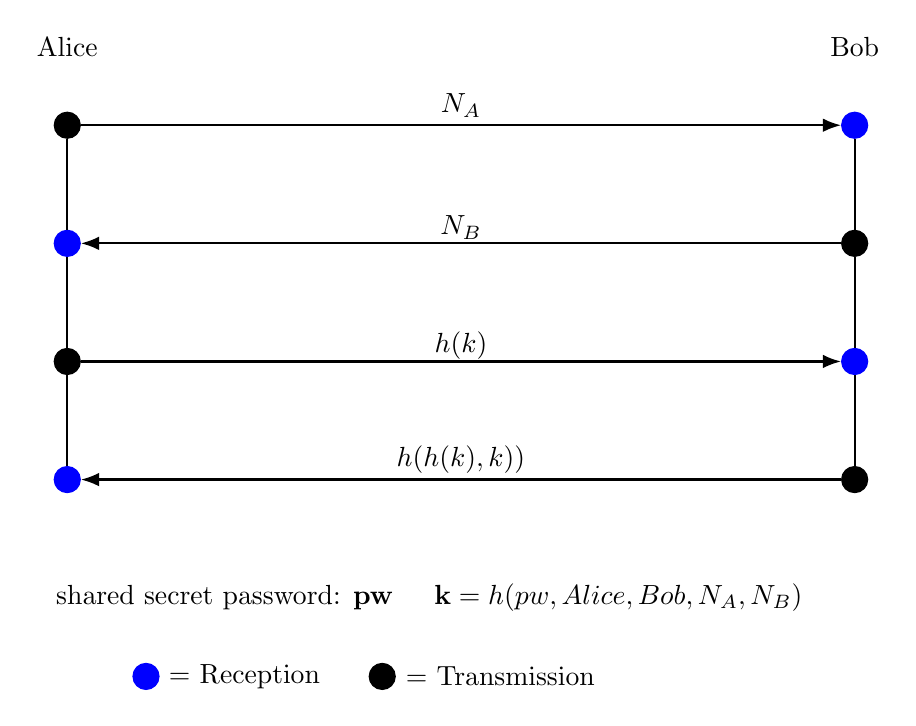
\begin{tikzpicture}
    \node at (0,8) {Alice};
    \node at (10,8) {Bob};
    \node[shape=circle,draw=blue, fill=blue] at (1,0) {};
    \node at (2.25,0) {= Reception};
    \node[shape=circle,draw=black, fill=black] at (4,0) {};
    \node at (5.5,0) {= Transmission};
    \node at (2,1) {shared secret password: \textbf{pw}};

    \pause
    \node[shape=circle,draw=black, fill=black] (1) at (0,7) {};
    \node[shape=circle,draw=blue, fill=blue] (2) at (10,7) {};
    \path [saiarrow](1) edge (2);
    
    \node at (5,7.25) {\(N_A\)};

    \pause
    \node[shape=circle,draw=black, fill=black] (3) at (10,5.5) {};
    \node[shape=circle,draw=blue, fill=blue] (4) at (0,5.5) {};
    
    \path [-,thick](3) edge (2);
    \path [saiarrow](3) edge (4);
    \path [-,thick](1) edge (4);
    
    \node at (5,5.7) {\(N_B\)};

    \pause
    \node[shape=circle,draw=black, fill=black] (5) at (0,4) {};
    \node[shape=circle,draw=blue, fill=blue] (6) at (10,4) {};
    
    \path [-,thick](6) edge (3);
    \path [saiarrow](5) edge (6);
    \path [-,thick](5) edge (4);
    
    \node at (5,4.2) {\(h(k)\)};
    \node at (7,1) {\(\mathbf{k} = h(pw,Alice,Bob,N_A,N_B)\)};
    
    \pause
    \node[shape=circle,draw=black, fill=black] (7) at (10,2.5) {};
    \node[shape=circle,draw=blue, fill=blue] (8) at (0,2.5) {};
    
    \path [-,thick](5) edge (8);
    \path [saiarrow](7) edge (8);
    \path [-,thick](6) edge (7);
    
    \node at (5,2.75) {\(h(h(k),k))\)};
    
\end{tikzpicture}
\end{frame}

\begin{frame}\frametitle{PAKE-0 textbook diagram}
\begin{figure}
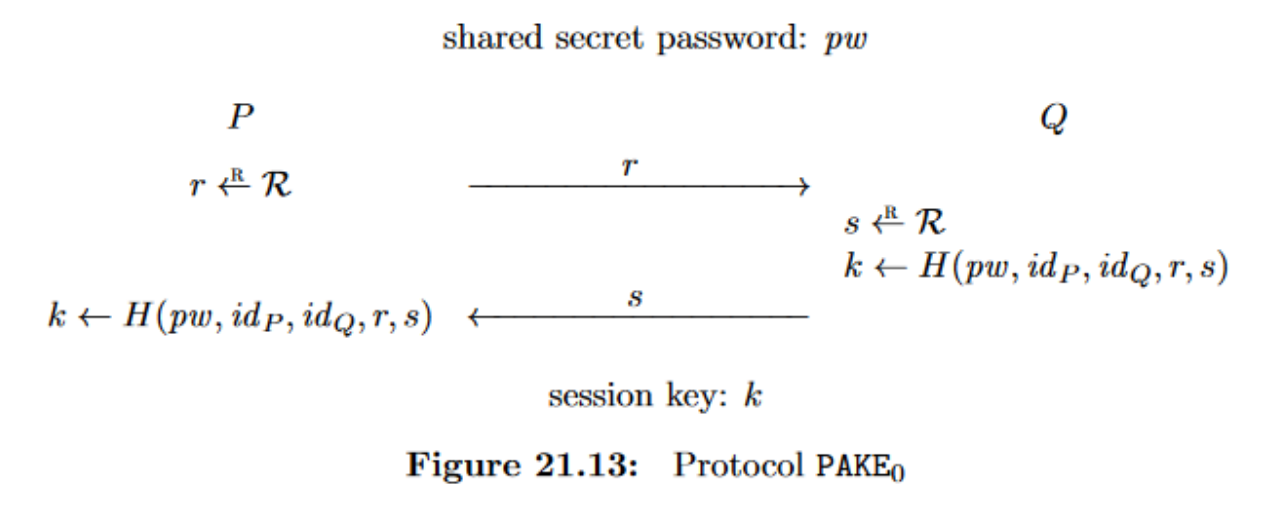
\includegraphics[width=\linewidth]{slide-images/pake-book}
\caption{Boneh, Dan, and Victor Shoup. "A graduate course in applied cryptography." Draft 0.5 (2020).}
\end{figure}
\end{frame}

\begin{frame}\frametitle{Assumptions in CPSA (1)}
Data origination assumptions:
\begin{itemize}
\item \textbf{uniq-orig} (e.g., nonce)
\end{itemize}
\begin{definition}[unique origination]
A value \emph{uniquely originates} in a bundle if it originates on exactly one strand. 
Note that if the unique origination point of a value is on a regular strand, then it cannot be produced in a ``create'' instance because that would constitute a second point of origination.
\end{definition}
\end{frame}

\begin{frame}\frametitle{Assumptions in CPSA (2)}
\begin{itemize}
\item \textbf{non-orig} (e.g., private key)
\end{itemize}
\begin{definition}[non-origination]
A value is \emph{non-originating} in a bundle if it does not originate on any strands. 
A simple lemma can show that a value is non-originating only if it is not carried in any message in the bundle.
\end{definition}
\end{frame}

\begin{frame}\frametitle{Assumptions in CPSA (3)}
\begin{itemize}
\item \textbf{pen-non-orig} (e.g., pre-shared password)
\end{itemize}
\begin{definition}[penetrator non-originating]
A value is \emph{penetrator non-originating} in a bundle of a protocol if it does not originate on any penetrator strands. 
Clearly, such a value cannot be produced in a ``create''
instance.
\end{definition}
\end{frame}

\begin{frame}\frametitle{Homework}
\pause
\begin{center}
{\Huge Model more in CPSA}
\end{center}
\pause
Now that you've seen PAKE modeled, can you model a more challenging protocol?

Model your meeting protocol from Homework 1!
\end{frame}

\begin{frame}\frametitle{Survey}
Fill in details about the survey here!
\end{frame}
\end{document}